\chapter{Kombinatorik} 

\section{Vereinigung und Kreuzprodukt von zwei Mengen} 

\begin{bem}
	Die Haupfrage der Kombinatorik ist ``Wie viele Elemente hat meine endliche Menge?''. Etwas formaler geht es um die Formeln für die Anzahl der Elemente verschiedener endlicher Mengen, welche man in der diskreten Mathematik gerne benutzt. 
\end{bem} 

\begin{lem} \label{lem:vereinigung:zwei}
	Seien $A, B$ endliche disjunkte Mengen. Dann ist $|A \cupdot B| = |A| + |B|$. 
\end{lem} 

\begin{proof}
	Ist $A$ oder $B$ leer, so gilt die Formel trivialerweise. Etwa, für $B = \emptyset$ gilt 
	\[
		|A \cup B| = | A \cup \emptyset| = |A| = |A| + 0 = |A| + | \emptyset| = |A| + |B|. 
	\]
	
	 Sonst nummerieren wir alle Elemente von $A$ als $a_1,\ldots,a_s$ und $B$ als $b_1,\ldots,b_t$. Das heißt, $A$ ist eine $s$-Elementige Menge $A = \{a_1,\ldots,a_s\}$ und $B$ ist eine $t$-elementige Menge $B = \{b_1,\ldots,b_t\}$ mit $s,t \in \N$. Es gilt $a_i \ne a_j$ für $i,j \in \{1,\ldots,s\}$ mit $i \ne j$   und $b_i \ne b_j$ für  $i,j \in \{1,\ldots,t\}$ mit $i \ne j$. Da $A$ und $B$ disjunkt sind gilt auch $a_i \ne b_j$ für alle $i \in \{1,\ldots,s\}$ und $j \in \{1,\ldots,t\}$. 
	 
	 Somit ist 
	 $A \cupdot B = \{a_1,\ldots,a_s,b_1,\ldots,b_t\}$, sodass wir $A \cupdot B = \{c_1,\ldots,c_n\}$ mit $n = s + t$ und 
	 \[
	 	c_i = \begin{cases}
	 		 a_i, & \text{für} \ i \in\{1,\ldots,s\}
	 		 \\b_{i-s}  &  \text{für} \ i \in \{s+1,\ldots,n\}
	 		\end{cases}.
 	\] 
 	Hierbei sind $c_1,\ldots,c_n$ nach der Konstruktion paarweise verschieden. Das zeigt, dass $A \cupdot B$ genau $n = s+t$ Elemente hat. 
\end{proof}

\begin{lem} \label{lem:disjunkte:vereinigung}
	Seien $A_1,\ldots,A_n$ ($n \in \N$) endliche paarweise disjunkte Mengen. Dann ist 
	\[
		\left| \bigcup_{i=1}^n A_i \right| = \sum_{i=1}^n |A_i|. 
	\]
\end{lem} 

\begin{proof} 
	Wir beweisen die die Formel durch Induktion über $n$. 
	Die Formel ist rivial für $n=1$, denn $\bigcup_{i=1}^1 A_i = A_1$ und $\sum_{i=1}^n |A_i|$ ist $|A_1|$. 
	Sei $n \in \N$ mit $n \ge 2$ gegeben und sei die Formel im Fall von $n-1$ an der Stelle von $n$ Mengen bereits verifiziert. Da die Mengen $A_1 \cup \cdots \cup A_{n-1}$ und $A_n$ paarweise disjunkt sind, erhalten wir durch die Anwendung von Lemma~\ref{lem:vereinigung:zwei} zu diesen beiden Mengen, dass 
	\[
		| A_1 \cup \cdots \cup A_n| = |A_1 \cup \cdots \cup A_{n-1} | + |A_n| 
	\]
	erfüllt ist. Aus der Induktionsvoraussetzung folgt, dass 
	\[
		| A_1 \cup \cdots \cup A_{n-1} | = \sum_{i=1}^{n-1} |A_i|
	\]
	erfüllt ist. Somit ist 
	\[
		| A_1 \cup \cdots \cup A_n| = \sum_{i=1}^{n-1} |A_i|  + |A_n| = \sum_{i=1}^n |A_i|. 
	\]
\end{proof} 

\begin{lem} \label{lem:inkl:exkl:2}
	Seien $A$ und $B$ endliche Mengen. Dann gilt 
	\[
		|A \cup B| = |A| + |B| - |A \cap B|. 
	\]
\end{lem}

\begin{proof}
		Wir können $A \cup B$ als dijsunkte Vereinigung von $A$ und $B \setminus A$ darstellen. Die Anwendung von Lemma~\ref{lem:vereinigung:zwei} zu $A$ und $B \setminus A$ ergibt 
		\[
			| A \cup B| = |A \cupdot (B \setminus A)| = |A | + |B \setminus A|. 
		\]
		Die Menge $B$ ist disjunkte Vereinigung von $B \setminus A$ und $A \cap B$. Die Anwendung von Lemma~\ref{lem:vereinigung:zwei} zu $A \cap B$ und $B \setminus A$ ergibt
		\[
			|B| = |B \setminus A| + |A \cap B|. 
		\]
		Aus den beiden Gleichungen, die wir auf diese Weise herleiten, folgt dann 
		\[
			| A \cup B|  = |A | + |B \setminus A| = |A| + (|B| - | A \cap B|) = |A| + |B| - | A \cap B|. 
		\]
\end{proof} 

\begin{bem}
	Die Intuition hinter Lemma~\ref{lem:inkl:exkl:2} ist: wir zählen alle Elemente in $A$ sowie $B$ ab. Dadurch werden die Elemente in $A \cap B$ doppelt abgezählt. Wir sollen also die Anzahl der Elemente in $A \cap B$ abbziehen, um auf die Anzahl der Elemente in $A \cup B$ zu kommen. 
\end{bem} 


\begin{bsp}
	Wie viele dreistellige Zahlen gibt es, bei denen zwei benachbarte Stellen gleich sind? 
	
	Wir identifizieren die dreistelligen Zahlen mit den  den Tripeln $(s_1,s_2,s_3)$ mit $s_1 \in \{1,\ldots,9\}$ und $s_2,s_3 \in \{0,\ldots,9\}$. Daher arbeiten wir innerhalb der Menge
	\[
			X = \{1,\ldots,9\} \times  \{0,\ldots,9\} \times \{0,\ldots,9\}
	\]
	Dann entspricht die Menge 
	\[
		A := \setcond{ (s_1,s_2,s_3) \in X}{s_1=s_2}
	\]
	der Menge der dreistelligen Zahlen, bei denen die $100$er und die $10$er Stelle gleich sind, und die Menge
	\[
		B:= \setcond{ (s_1,s_2,s_3)}{s_2=s_3}
	\]
	der Menge der dreistelligen Zahlen, bei denen die $10$er und die $1$er Stelle gleich sind. Wir sind also an der Anzahl der Elemente in der Vereinigung $A \cup B$ interessiert. Wegen 
	\[
			| A \cup B| = |A| + |B|  - |A \cap B|
	\]
	reicht es aus, die Anzahl der Elemente in $A$, $B$ und $A \cap B$ zu bestimmen. 	
	Der Durchschnitt 
	\[	
		A \cap B = \setcond{ (s_1,s_2,s_3) \in X}{s_1=s_2=s_3}
	\]
	entspricht der Menge der dreistelligen Zahlen, bei denen alle drei Stellen gleich sind. Die Menge $A$ hat genau $9 \cdot 10$ Elemente. Das lässt sich folgendermaßen verifizieren:  
	\begin{itemize} 
		\item es gibt für die $100$er Stelle $9$ Möglichkeiten hat;
		\item unabhängig von der $100$er Stelle gibt es für die $1$er Stelle $10$ Möglichkeiten
		\item Die $10$er Stelle bei den Zahlen, die den Elementen aus $A$ entsprechen, ist gleich der $100$er Stelle. 
	\end{itemize} 
	Ganz analog sieht man, dass die Menge $B$ ebenfalls genau $9 \cdot 10$ Elemente hat. Die Menge $A\cap B$ hat $9$ Elemente. Es folgt: 
	\[
		|A \cup B| = 90 + 90 - 9 = 171. 
	\]	
	Hier ein Python-Code, der all die Möglichkeiten auflistet: 
	\lstinputlisting{Code/komb171.py}
\end{bsp} 


\begin{bsp}
	In einer Klasse haben $15$ Kinder eine Playstation, $10$ Kinder eine Xbox und $3$ Kinder die beiden genannten Geräte. Wie viele Kinder haben mindestens eines der beiden Geräte? 
	
	Sei $P$ die Menge der Kinder, die eine Playstation haben, $X$ die Anzahl der Kinder, die eien Xbox haben. Dann gilt: 
	\[
		|P \cup X| = |P| + |X| - |P \cap X| = 15 + 10 - 3 = 22. 
	\]
\end{bsp} 

\begin{bem}[Kombinatorik und Wahrscheinlichkeiten] 
	Die Berechnung von Wahrscheinlichkeiten reduziert sich im Fall von endlichen Wahrscheinlichkeitsräumen oft zur Berechnung von Quotienten 
	\begin{align*}
			\frac{\text{die Anzahl der günstigen Fälle}}{\text{die Anzahl aller Fälle}}
	\end{align*} 
	uns somit zur Lösung von kombinatorischen Aufgaben, vgl. auch \cite{Tit19}. 
\end{bem} 

\begin{aufg}
	Alice wirft zwei Spielwürfel und Bob wirft einen Spielwürfel. Mit welcher Wahrscheinlichkeit ist die Augenzahl bei Bob gleich einer der Augenzahlen bei Alice? 
\end{aufg} 

\begin{lem} \label{lem:anzahl:prod:2}
	Seien $A$ und $B$ endliche Menge. Dann gilt: 
	\[
		|A \times B| = |A| \cdot |B|. 
	\]
\end{lem}
\begin{proof} 
	Ist $A$ oder $B$ leer, so sind die linke sowie rechte Seite der Gleichung gleich $0$. Ansonsten stellen wir die Menge $A \times B$ kann als disjunkte Vereinigung $\bigcup_{a \in A} \{a\} \times B$ da. Lemma~\ref{lem:disjunkte:vereinigung} ergibt
	\[
		|A \times B| = \left| \bigcup_{a \in A} \{a \} \times B \right| = \sum_{a \in A} | \{a \} \times B |.
	\]
	Für ein beliebiges festes $a \in A$ kann nun die Anzahl der Elemente in $\{a\} \times B$ bestimmt werden. Diese Anzahl ist $|B|$, da die Abbildung $f_a : B \to \{a\} \times B$ mit $f_a(b) := (a,b)$ bijektiv ist: denn hat man zwei verschiedene Elemente $b',b'' \in B$ so sind auch $(a,b')$ und $(a,b'')$ verschieden (Injektivität) und hat man ein beliebiges Element aus $\{a\} \times B$ fixiert, etwa $(a,b)$ mit $b \in B$, so erhält man dieses Element als $f_a(b) = (a,b)$. 
\end{proof} 

\begin{bsp}
	In einem Kinosaal hat man $10$ Reihen mit $16$ Plätzen pro Reihe. Jeder Platz kann also durch die Angabe der Reihe und die Nummer des Platzes in der Reihe als das Paar $(r,n)$ mit $r \in \{1,\ldots,10\}$ und $n \in \{1,\ldots,16\}$ notiert werden. Die Anzahl der Plätze ist 
	\[
			| \{1,\ldots,10\} \times \{1,\ldots,16\} |  = | \{1,\ldots,10\} | \times | \{1,\ldots,16\}| = 10 \cdot 16 = 160. 
	\]
	Dieses Beispiel ist genauso einfach wie unser Lemma~\ref{lem:anzahl:prod:2}, das die Idee hinter dem Beispiel ganz allgemein erfasst. 
\end{bsp} 
 

\section{Kartesisches Produkt} 

\begin{thm} \label{thm:kreuz:produkt}
	Seien $A_1,\ldots, A_n$ endliche Mengen ($n \in \N$). Dann ist 
	\[
		|A_1 \times \cdots \times A_n|  = \prod_{i=1}^n |A_i|. 
	\]
\end{thm} 
\begin{proof}
	Wir beweisen die Gleichung durch Induktion über $n$.
	Für $n=1$ erhalten wir eine triviale Identät. Sei die Gleichung für $n-1$ Mengen für ein $n \in \N$ mit $n \ge 2$ efüllt. Dann erhält man wegen 
	\[
			A_1 \times \cdots \times A_n = A_1 \times (A_2 \times \cdots \times A_n)
	\]
	durch die Anwendung von Lemma~\ref{lem:anzahl:prod:2} die Gleichung 
	\[
		|A_1 \times \cdots \times A_n | = |A_1| \cdot |A_2 \times \cdots \times A_n|. 
	\]
	Anschließend erhalten wir aus der Induktionsvoraussetzung 
	\[
		|A_2 \times \cdots \times A_n| = \prod_{i=2}^n |A_i|,
	\]
	woraus sich die gewünschte Gleichung für die Mengen $A_1,\ldots,A_n$ ergibt. 
\end{proof} 

\begin{bem}[Identifikation  in der Mathematik: das Selbe oder das Gleiche?]
	In der Mathematik wird oft eine stillschweigende Identifikation von Objekten vorgenommen. Genauer sind  zwischen manchen paaren von Mengen natürliche Bijektionen vorhanden, auf deren Basis diese Mengen identifiziert werden. Zum Beispiel kann man für eine Menge $X$ die kartesische erste Potenz $X^1$ mit $X$ identifizieren, weil man ein einelementiges Tupel $(x)$ mit $x \in X$ mit $x \in X$ identifizieren kann. Man geht also davon aus, dass $(x)$ das Selbe wie $x$ ist. Beim Programmieren dagegen erfolgt eine solche Identifikation nicht immer automatisch: man soll dann Objekte verschiedener Datentypen explizit in einander konvertieren. 
	
	Im vorigen Beweis haben wir $(a_1,(a_2,\ldots,a_n))$, ein Paar, bei dem die zweite Komponente ein $(n-1)$-Tupel ist, stillschweigend mit $(a_1,\ldots,a_n)$ identifiziert. 
\end{bem} 

\begin{kor} \label{kor:product} 
	Sei $A$ endliche Menge und $n \in \N$. Dann gilt $|A^n| = |A|$. 
\end{kor}
\begin{proof}
	Die Behauptung folgt durch die Anwendung von Theorem~\ref{thm:kreuz:produkt} im Fall, dass alle Mengen $A_1,\ldots,A_n$ gleich $A$ sind. 
\end{proof}  

\section{Abbildungen} 

\begin{thm}
	Seien $X,Y $ endliche Mengen. Dann gilt $|Y^X| = |Y|^{|X|}$, wobei man bei $X= Y = \emptyset$, $|Y|^{|X|} = 0^0  =1$ setzt. 
\end{thm}
\begin{proof}
	Im entarteten Fall $X = \emptyset$ gibt es nur eine Abbildung von $\emptyset$ nach $Y$. 
	Sei $X \ne\emptyset$ und sei $n := |X|$, sodass wir alle Elemente von $x$ als $x_1,\ldots,x_n$ indexieren können. Dann entspricht jede Abbildung $f : X \to Y$ einem $n$-Tupel $(f(x_1),\ldots,f(x_n)) \in Y^n$, wobei zwei verschiedene Abbildungen von $X$ nach $Y$ zwei verschiedene Tupel erzuegen. 
	Umkgekehrt definiert jedes $n$-Tupel $(y_1,\ldots,y_n)$ die Abbildung $f: X \to Y$ mit $f(x_i)  = y_i$ für alle $i \in \{1,\ldots,n\}$. Man sieht also, dass die Abbildung 
	\[
			Y^X \to Y^n,
	\]
	die einem $f : X \to Y$ das Tupel $(f(x_1),\ldots,f(x_n))$ zuordnet, bijektiv ist. Wir erhalten mit der Verwendung von Korollar~\ref{kor:product}
	\[
			|Y^X| = |Y^n| = |Y|^n = |Y|^{|X|}. 
	\]
\end{proof} 

\begin{bsp}
	Wieviele Möglichkeiten gibt es drei verschiedene Aufgaben unter vier Personen zu verteilen, wenn jede Aufgabe genau einer Personen zugeordent wird? 
	
	Eine Zuordnung der Aufgaben den Personen ist eine Abbildung aus einer $3$-elementigen Menge $X$ von  Aufgaben in die $4$-elementige Menge $Y$ der Personen. Wir zählen also die Abbildungen aus $Y^X$. Die Anzahl ist $|Y^X| = |Y|^{|X|} = 4^3 = 64$. 
\end{bsp} 

\begin{bem}\
	\lstinputlisting{Code/Abb.py} 
	Demo dazu: 
	\lstinputlisting{Code/Abb_demo.py}
\end{bem}

\section{Injektive und bijektive Abbildungen} 

\begin{defn}[Fakultät]
	Für $n \in \N_0$ ist \textbf{$n$ Fakultät} als 
	\[n ! := \prod_{i=1}^n i
	\] definiert. Insbesondere gilt $0!=1!=1$. 
\end{defn} 

\begin{defn}
	Für $n, k \in \N_0$ definieren wir die \textbf{fallende Faktorielle} von $n$ der Länge $k$ als
	\[
		n^{\underline{k}} := n \cdot \ldots \cdot (n-k+1).
	\]
	Man hat insbesondere $n^{\underline{0}}=1$. 
\end{defn} 

\begin{defn}
	Für Mengen $X, Y$ bezeichnen wir als $\Inj(X,Y)$ die Menge aller injektiven und als $\Bij(X,Y)$ die Menge aller bijektiven Abbildungen von $X$ nach $Y$. 
\end{defn} 

\begin{thm} \label{thm:inj:abbildungen}
	Seien $X,Y$ endliche Mengen. Dann ist $|\Inj(X,Y) | = |Y|^{\underline{|X|}}$. 
\end{thm} 
\begin{proof} 
	Wenn es eine injektive Abbildung $f$ von $X$ existiert $Y$ exisitert, so gilt $|X| \le |Y|$, denn $f(X)$ ist eine Teilmenge von $Y$, die genau so viele Elemente wie $X$ hat. Das bedeutet, dass die Formel iim $|X| > |Y|$ erfüllt ist, weil in diesem Fall die linke sowie rechte Seite gleich $0$ ist. Wir beweisen die Formeln im Fall $|X| \le |Y|$ durch Induktion über $|X|$. Für $X = \emptyset$ gibt es genau eine injektive Abbildung von $X= \emptyset$ nach $Y$. Also gilt die Formel für $|X|=0$. 
	Nun betrachten wir $X$ und $Y$ mit $k=|X|$ und $k \le |Y|$ und nehmen an, dass die Formel im Fall $k-1=|X| \le |Y|$ bereits verifiziert wurde. Wir fixieren ein beliebiges $a \in X$. Jede injektive Abbildung $f$ von $X$ nach $Y$ bildet das fixierte $a$ auf eines der Elemente aus $Y$ ab. Wir können also die Menge $\Inj(X,Y)$ als disjunkte Vereinigung 
	\[
			\Inj(X,Y) = \bigcup_{b \in Y} \Inj_{a,b}(X,Y),
	\]
	mit 
	\[
		\Inj_{a,b} (X,Y) := \setcond{ f \in \Inj(X,Y)}{f(a) = b}. 
	\]
	Nach Lemma~\ref{lem:disjunkte:vereinigung} gilt 
	\[
			|\Inj(X,Y)| = \sum_{b \in Y} |\Inj_{a,b}(X,Y)|
	\]
	Jede Abbildung $f  \in \Inj_{a,b}(X,Y)$ erzeugt die Abbildung $\tilde{f} : X \setminus \{a\} \to Y \setminus \{b\}$. Da $f$ injektiv ist, ist $\tilde{f}$ ebenfalls injektiv. Auf diese Weise haben wir die Abbildung 
	\[
				f \mapsto \tilde{f} 
	\]
	von $\Inj_{a,b}(X,Y)$ nach $\Inj(X \setminus \{a\}, Y \setminus \{b\})$ erstellt. Die Abbildung $f$ ist offensichtlich eine Bijektion, sodass man $|\Inj_{a,b}(X,Y)| = |\Inj(X \setminus \{a\},Y \setminus \{b\})|$ hat. Nach der Induktionsvoraussetzung ist 
	\[
		|\Inj(X \setminus \{a\}, Y \setminus \{b\} | = |Y \setminus \{b\}|^{\underline{|X \setminus \{a\}}} = (|Y| -1)^{\underline{|X|-1}}.
	\] 
	Es folgt 
	\begin{align*}
	|\Inj(X,Y)| & = \sum_{b \in Y} |\Inj_{a,b}(X,Y)| 
		\\ & = \sum_{b \in Y} (|Y| -1)^{\underline{|X|-1}} 
		\\ & = |Y| \cdot (|Y| -1)^{\underline{|X|-1}}
		\\ & = |Y|^{\underline{|X|}}. 
	\end{align*}
\end{proof} 

\begin{bsp}
		In einer Deutsch-Stunde sollen  $3$ von $25$ Schüler:innen ein Gedicht vortragen. Wie viele Möglichkeit gibt es dafür, wenn man die Reihenfolge, in der man vorträgt, berücksichtigt? Wir zählen injektive Abbildungen von $\{1,2,3\}$ in die Menge der $25$ Schüler:innen. Die Antwort: 
		\[
			25^{\underline{3}} = 25 \cdot 24 \cdot 23. 
		\]
\end{bsp} 

\begin{bem}\
\lstinputlisting{Code/Inj.py} 
\end{bem}

\begin{kor}
	 Seien $X$ und $Y$ endliche Mengen der gleichen Kardinalität $n$. Dann gilt $|\Bij(X,Y)| = n!$
\end{kor} 
\begin{proof}
	Haben endliche Mengen $X$ und $Y$ die gleiche Kardinalität, so gilt die Gleichheit $\Bij(X,Y ) = \Inj(X,Y)$. Die Inklusion $\Bij(X,Y ) \subseteq \Inj(X,Y)$ ist trivial, weil jede Abbildung nach der Definition injektiv ist. Umgekehrt: Ist $f: X \to Y$ injektiv, so hat $Y \setminus f(X)$ genau $|Y| - |f(X)| = |Y| - |X| =0$ Elemente. Das bedeutet, $Y = f(X)$, sodass $f$ auch surjektiv ist. Das zeigt die Inklusion $\Inj(X,Y) \subseteq \Bij(X,Y)$. 
	
	Nach dieser Bemerkung folgt die Behauptung direkt aus Theorem~\ref{thm:inj:abbildungen}. 
\end{proof} 

\begin{bsp}
	Wie viele Möglichkeiten gibt es, $10$ verschiedene Bücher in einem Regal anzuordnen? Wir zählen bijektive Abbildungen von $\{1,\ldots,10\}$ in die Menge von $10$ Büchern. Die Antwort: 
	\[
			10!
	\]
\end{bsp} 

\begin{bem} Der Demo-Code 
\lstinputlisting{Code/Inj_demo.py}
ergibt $6$ Möglichkeiten. 
\end{bem} 

\begin{aufg}[Geburtstage]\
	\begin{enuma}
		\item Mit welcher Wahrscheinlichkeit haben $2$ zufällig gewählte Personen den gleichen Geburtstag? 
		\item Mit welcher Wahrscheinlichkeit gibt es unter $3$ zufällig gewählten Personen zwei mit dem gleichen Geburstag?
		\item Mit welcher Wahrscheinlichkeit gibt es unter $25$ zufällig gewählten Personen zwei mit dem gleichen Geburstag?
		\item Mit welcher Wahrscheinlichkeit gibt es unter $366$ zufällig gewählten Personen zwei mit dem gleichen Geburstag? 
	\end{enuma}
	Bemerkung: Wir ignorieren Einfachheit halber die Problematik mit den Schaltjahren und gehen davon aus, dass das Jahr $365$ hat. 
\end{aufg} 

\section{Teilmengen} 

\begin{defn}
Für eine Menge $X$ xund $k \in \N_0$ bezeichnen wir als $\binom{X}{k}$ die Menge aller $k$-elementigen Teilmengen von $X$. 
\end{defn}

\begin{bsp}
	\[
	\binom{\{1,2,3,4\}}{2} = \Bigl\{ \{1,2\},\{1,3\}, \{1,4\}, \{2,3\}, \{2,4\} ,\{3,4\} \Bigr\}.
	\]
\end{bsp} 


\begin{defn}
	Für $n,k \in \N_0$ wird der \textbf{Binomialkoeffizient  $n$ über $k$} als 
	\[
		\binom{n}{k}:= \frac{n^{\underline{k}}}{k!}  = \frac{n \cdot \ldots \cdot (n-k+1)}{k!}.
	\]
	definiert. 
\end{defn} 

\begin{bem}
	Im Fall $0 \le k \le n$ und $n,k \in \N_0$ hat man $\binom{n}{k} = \frac{n!}{k! (n-k)!}$. 
\end{bem} 


\begin{thm} \label{thm:k:elem:teilmengen} 
		Sei $X$ endliche Menge und sei $k \in \N_0$. Dann gilt: 
		\[
				\left| \binom{X}{k} \right| = \binom{|X|}{k}. 
		\]
\end{thm} 
\begin{proof} 
	In den Fällen $k > |X|$ werden die beiden Seiten der Formel gleich $0$. Wir nehmen also $k \le |X|$ an. Ist $k=0$, werden die beiden Seiten der Formeln gleich $1$. Wir nehmen also $0 < k \le |X|$ an. 
	
	Wir zählen die injektiven Abbildungen von $I:=\{1,\ldots,k\}$ nach $X$ auf die folgende  Weise auf. Bei jeder injektiven Abbildung $f : I \to X$ ist das Bild $f(I)$ eine $k$-elementige Teilmenge von $X$. Also kann man die injektiven Abbildungen $f: I \to X$  nach der Wahl von $f(I)$ gruppieren. Mit anderen Worten ist $\Inj(I,X)$ disjunkte Vereinigung
	\[
		\Inj(I,X)  = \bigcup_{B \in \binom{X}{k} } \setcond{f \in \Inj(I,X)}{f(I) = B}. 
	\]
	Aus Lemma~\ref{lem:disjunkte:vereinigung} folgt
	\[
		|\Inj(I,X) | = \sum_{B \in \binom{X}{k} } | \setcond{f \in \Inj(I,X)}{f(I) = B}|. 
	\]
	Jeder ijectiven Abbildung $ f: I \to X$ mit einem vorgeschriebenen Bild $B$ 
	die bijektive Abbildung $\tilde{f} : I \to B$ mit $\tilde{f}(i) = f(i)$ zuordnen kann, und die Abbildung $f \mapsto \tilde{f}$ von $\setcond{f \in \Inj(I,X)}{f(I) = B}$ nach $\Bij(I,B)$ ist bijektiv. 
	Wir erhalten also 
	\[
			| \setcond{f \in \Inj(I,X)}{f(I) = B}| = |\Bij(I,B)| = k!
	\]
	Das ergibt
	\[
		|\Inj(I,X) | = \left| \binom{X}{k} \right| \cdot k!
	\]
	Nach Theorem~\ref{thm:inj:abbildungen} hat man 
	\[
		|\Inj(I,X)| = |X|^{\underline{k}}. 
	\]
	Es folgt: 
	\[
		\left| \binom{X}{k} \right| = \frac{|\Inj(I,X) |}{k!} = \frac{|X|^{\underline{k}}}{k!} = \binom{|X|}{k!}. 
	\]
\end{proof} 

\begin{bem}[Doppeltes Abzählen] 
	Im Beweis des  Theorems~\ref{thm:k:elem:teilmengen} haben wir injektive Abbildungen zwischen zwei festgelegten Mengen auf eine andere Weise als im Beweise des Theorems~\ref{thm:inj:abbildungen} abgezählt. Aus den beiden Weisen abzuzählen ergab sich dann im Beweis des Theorems~\ref{thm:inj:abbildungen} für die Anzahl der $k$-elementigen Teilmengen einer gegebenen Menge. Solchen Beweisansatz nennt man in der Kombinatorik \textbf{Doppeltes Abzählen}. 
\end{bem} 

\begin{aufg}
	Für alle $n,k \in \N_0$ gilt $\binom{n}{k} = \binom{n}{n-k}$. Verifizieren Sie das direkt arithmetisch und kombinatorisch, indem man eine Bijektion zwischen 
	den Mengen $\binom{X}{k}$ und $\binom{X}{|X|-k}$ für eine $n$-elementige Teilmenge $X$ erstellt. 
\end{aufg} 


\begin{thm}
	Sei $X$ endliche Menge. Dann gilt $|2^X|=2^{|X|}$. 
\end{thm} 
\begin{proof} 
	Es gibt verschiedene Ansätze zum Beweis dieser Formel. Zum Beispiel kann man eine natürliche Bijektion zwischen  $2^X$ und $\{0,1\}^X$ erstellen und dann $|\{0,1\}^X| = |\{0,1\}|^{|X|} = 2^{|X|}$ nutzen (Aufgabe). 
	
	Wir präsentieren hier einen Beweis durch Induktion über $|X|$. Hat $X$ $0$ Elemente, so gilt $2^X = 2^\emptyset = \{\emptyset\}$. Somit ist $|2^X| = 1 = 2^0 = 2^{|X|}$. Sei $X$ Mengen mit $n$ Elementen, mit $n \ge 1$, und sei die Formel für Mengen $X$ mit $n-1$ Elementen bereits verifiziert. Wir fixieren ein $a \in X$. Die Teilmengen $A$ von $X$ zerlegen sich nach den Bedingungen $a \in A$ und $a \not\in A$ in zwei disjunkte Mengen. Es gilt also
	\begin{align*}
			2^X & = \setcond{A}{A \subseteq X, \ a \in A} \cupdot \setcond{A}{A \subseteq X, \ a \not\in A}
			\\ & = \setcond{B \cup \{a\}}{B \subseteq X \setminus \{a\}} \cupdot 2^{X \setminus \{a\}}. 
	\end{align*}
	Das ergibt
	\[
		|2^X| = |\setcond{B \cup \{a\}}{B \subseteq X \setminus \{a\}}| + | 2^{X \setminus \{a\}}|. 
	\]
	Die Abbildung $B \mapsto B \cup \{a\}$ ist eine Bijektion von $2^{X \setminus \{a\}}$ nach $\setcond{B \cup \{a\}}{B \subseteq X \setminus \{a\}}$. Es folgt: 
	\[
		|2^X| = 2 \cdot |2^{X \setminus \{a\}}|
	\]
	Da $X \setminus \{a\}$ eine $(n-1)$-elementige Menge ist, folgt nach der Induktionsovraussetzung $|2^{X \setminus \{a\}}| = 2^{|X \setminus \{a\}|} = 2^{|X|-1}$. Wir erhalten somit $|2^{X}| = 2 \cdot 2^{|X|-1} = 2^{|X|}$. 
\end{proof} 

\begin{bem} Aufzählungscode der dem vorigen Beweis entspricht: 
\lstinputlisting{Code/Teilmengen.py}
\end{bem} 

\begin{aufg}
	Wie wahrscheinlich ist es, beim viermaligen Werfen einer fairen Münze, genau $2$ mal den Kopf zu werfen?
\end{aufg} 



\begin{thm}[Binomialsatz] 
	Für $x, y \in \R$ und $n \in \N$ gilt 
	\[
			(x+y)^n = \sum_{i=0}^n \binom{n}{i} x^i y^{n-i}. 
	\]
\end{thm} 
\begin{proof}
	Es gibt einen direkten kombinatorischen Beweis dieser Formel. Beim Auflösen der Klammern im Ausdruck 
	\[
			(x+y)^n = \underbrace{(x+y) \cdots \ldots \cdot (x+y)}_{n \ \text{mal}}
	\]
	erhält man $2^n$ Terme, indem man aus jeder der $n$ Klammern $x$ oder $y$ wählt und die so gewählten Werte miteinander multipliziert. Wenn wir durch $I$ die Nummern der Klammern bezeichnen, aus denen der Wert $x$ gewählt wurde, erhalten wir 
	\[
			(x+y)^n = \sum_{I \subseteq \{1,\ldots,n\}} x^{|I|} y^{n - |I|}. 
	\]
	Anschließend gruppieren wir die Teilmengen $I \subseteq \{1,\ldots,n\}$ nach ihrer Kardinalität und erhalten
	\begin{align*}
			(x+y)^n & =\sum_{i=0}^n \sum_{I \in \binom{\{1,\ldots,n\}}{i}} x^i y^{n-i} 
			\\ & = \sum_{i=0}^n \left| \binom{\{1,\ldots,n\}}{i} \right| x^i y^{n-i} 
			\\ & = \sum_{i=0}^n \binom{n}{i}  x^i y^{n-i}.
	\end{align*} 
\end{proof} 

\begin{thm} \label{pascals:triangle} 
	Für alle $n \in \N$ und $i \in \N_0$ hat man $\binom{n}{i}  = \binom{n-1}{i}  + \binom{n-1}{i-1}$. 
\end{thm} 
\begin{proof} 
	Wir beschränken uns auf den nichttrivialen Fall $1 \le i \le n$. 
	
	Man kann für die Formel in der Behauptung einen rein arithmetischen Beweis anhand der expliziten Formel für die Binomailkoeffizienten geben. 
	
	Alternativ geben wir hier einen kombinatorischen Beweis. Sei $X$ eine $n$-elementige Menge. Wir fixieren ein Element $p\in X$ in dieser Menge. Die Menge $\binom{X}{i}$ der $i$-elementigen Teilmengen ist disjunkte Vereinigung 
	\[
		\binom{X}{i} = \setcond{ A \in \binom{X}{i}}{p \in A} \cupdot \setcond{A \in \binom{X}{i}}{p \not\in A}. 
	\]
	Hierbei ist 
	\[
			\setcond{A \in \binom{X}{i}}{p \not\in A} = \binom{X \setminus \{p\}}{i}
	\]
	und $\setcond{ A \in \binom{X}{i}}{p \in A}$ kann bijektiv auf 
	\[
			\binom{X \setminus \{p\}}{i-1}
	\]
	abgebildet werden, indem man $A$ auf $A \setminus \{p\}$ abbildet. Auf diese Weise erhält man 
	\begin{align*}
		\binom{n}{i} = \left| \binom{X}{i} \right| & = \left| \binom{X \setminus \{p\}}{i} \right| + \left| \binom{X \setminus \{p\}}{i-1}\right| 
		\\ & = \binom{n-1}{i} + \binom{n-1}{i-1}. 
	\end{align*} 
\end{proof} 

\begin{aufg}
	Die Formel in Theorem~\ref{pascals:triangle} wird oft als das sogenannte pascalsche Dreieck visualisiert. 
	\begin{center}
	\begin{tabular}{rrrrrrrrr}
1\\
1 & 1\\
1 & 2 & 1\\
1 & 3 & 3 & 1\\
1 & 4 & 6 & 4 & 1\\
1 & 5 & 10 & 10 & 5 & 1\\
1 & 6 & 15 & 20 & 15 & 6 & 1\\
1 & 7 & 21 & 35 & 35 & 21 & 7 & 1\\
1 & 8 & 28 & 56 & 70 & 56 & 28 & 8 & 1
	\end{tabular}
\end{center}
Schauen Sie sich das Dreieck an. Versuchen Sie darauf basierend die Ausdrückie wie $(x+y)^6$ oder zum Beispiel $(x+y)^9$ auszumultiplizieren. 
\end{aufg} 

\begin{aufg}
	Beweisen Sie den binomischen Lehrsatz durch Induktion über $n$ mit der Verwendung von Theorem~\ref{pascals:triangle}. 
\end{aufg} 

\section{Das Prinzip der Inklusion-Exklusion} 

\begin{defn}
	Seien $A,X$ Mengen mit $A \subseteq X$. Dann nennen wir die Funktion $1_A : X \to \R$ mit 
	\[
		1_A(x): = \begin{cases}
				1 &  \text{für} \ x \in A, 
			\\	0 & \text{für} \ x \not\in A
			\end{cases} 
	\]
	die \textbf{charakteristische Funktion} von $A$ auf der Grundmenge $X$. 
	
	In der Regel ist die Wahl der Grundmenge aus dem Kontext klar, daher ist $X$ nicht direkt in der Bezeichnung $1_A$ vorhanden.
\end{defn} 

\begin{bem}
	Andere Bezeichnungen für die charakteristische Funktion von $A$, die man in der Literatur benutzt, sind $f_A$, $\chi_A$ und $[A]$. Die charakteristische Funktion wird auch die \textbf{Indikator-Funktion} genannt. 
\end{bem} 

\begin{bem}
	Sind $A, X$ endliche Menge mit $A \subseteq X$ so ist 
	\[	
			|A| = \sum_{x \in A} 1_A(x)
	\] 
	Darüber hinaus gilt 
	\[	
		1_{X \setminus A} = 1_X - 1_A. 
	\]
\end{bem}

\begin{lem}
	Seien $A_1,\ldots,A_n$ ($n \in \N$) endliche Teilmengen einer endlichen Menge $X$. Dann gilt 
	\[
			1_{A_1 \cap \cdots \cap A_n}  = 1_{A_1} \cdot \ldots \cdot 1_{A_n}. 
	\]
\end{lem} 
\begin{proof}
	Sei $x \in X$. 
	Liegt $x$ im Durchschnitt der Mengen $A_1,\ldots,A_n$ so gilt 
	\[ 1_{A_1 \cap \cdots \cap A_n} (x) =1
	\]  aber auch $1_{A_i}(x)=1$ für jedes $i \in \{1,\ldots,n\}$. Die Auswertung der Funktionen auf der linken und rechten Seite auf $x$  ergibt somit den Wert $1$
	Ist $x$ nicht im Durchschnitt der Mengen $A_1,\ldots,A_n$ so gilt $1_{A_1 \cap \cdot A_n}(x) =0$ aber auch $1_{A_i}(x)=1$ für ein $i \in \{1,\ldots,n\}$. Die Auswertung der Funktionen auf der linken rechten Seite der Formel ergibt somit den Wert $0$. 
\end{proof} 

\begin{lem} \label{lem:product} 
	Sei $n \in \N$. Dann gilt für alle $t_1,\ldots,t_n \in \R$ die Gleichung 
	\[
		(1 - t_1) \cdot \ldots \cdot  (1-t_n) = \sum_{I \subseteq \{1,\ldots,n\}} (-1)^{|I|} \prod_{i \in I} t_i.  
	\]
	(Deutung der rechten Seite: die Summe über alle Teilmengen $I$ von $\{1,\ldots,t\}$ und das Produkt aller $t_i$ mit $i \in I$). 
\end{lem} 
\begin{proof} 
	Die Gleichung folgt durch das Ausmultiplizieren. Aus jeder der $n$ Klammern au fer linken Seite der Formel kann  beim Ausmultiplizieren unabhängig der Term $1$ oder der Term $-t_i$ gewählt werden. Die Menge $I$ kodiert also die Wahl der Terme in den Klammern durch die Angabe der Klammern, in denen man den Term $-t_i$ gewählt hat. Man hat also 
	\[
			(1 - t_1) \cdot \ldots \cdot  (1-t_n) = \sum_{I \subseteq \{1,\ldots,n\}}  \prod_{i \in I} (-t_i)  = \sum_{I \subseteq \{1,\ldots,n\}} (-1)^{|I|} \prod_{i \in I} t_i.
	\]
	Einen formaleren Beweis kann man zum Beispiel durch Induktion über $n$ führen (Aufgabe). 
\end{proof} 

\begin{thm}[Das Prinizip der Inklusion-Exklusion]
	Seien $A_1,\ldots,A_n$ ($n \in \N$) endliche Mengen. Dann gilt 
	\[
		| A_1 \cup \cdots \cup A_n| = \sum_{\emptyset \ne J \subseteq \{1,\ldots,n\}} (-1)^{|J|+1} \left| \bigcap_{j \in J} A_i \right| 
	\]
\end{thm} 
\begin{proof} 
	Wir setzen $X := A_1 \cup \cdots \cup A_n$ und betrachten die charakteristischen Funktionen von $A_1,\ldots,A_n$ auf der Grundmenge $X$. Dann gilt die Identität
	\[
		  (1-1_{A_1} )  \cdots (1 -1_{A_n}) = 0
	\]
	auf der Menge $x$; denn für jedes $x \in X$ hat man $x \in A_i$ für ein $i \in \{1,\ldots,n\}$, woraus sich $1 - 1_{A_i}(x) = 0$ ergibt. 
	
	Aus Lemma~\ref{lem:product} folgt dann 
	\[
		 0 = \sum_{I \subseteq \{1,\ldots,n\}} (-1)^{|I|} \prod_{i \in I} 1_{A_i} = \sum_{i \in I} (-1)^{|I| } \, 1_{\bigcap_{i \in I} A_i},
	\]
	wobei wir hier $\bigcup_{i \in \emptyset} A_i$ als $X$ interpretieren. 
	Daraus folgt: 
	\begin{align*}
		0  & = \sum_{x \in X} \sum_{i \in I} (-1)^{|I| } \, 1_{\bigcap_{i \in I} A_i}(x)
		\\ & = \sum_{I \subseteq \{1,\ldots,n\} } (-1)^{|I| } \sum_{x \in X} 1_{\bigcap_{i \in I} A_i}(x)
		\\ & = \sum_{I \subseteq \{1,\ldots,n\}} (-1)^{|I| } \left| \bigcap_{i \in I} A_i \right|
	\end{align*}
	Wir spalten in der vorigen Summer den Summanden zu $I = \emptyset$ ab und erhalten 
	\[
		0  = |X| + \sum_{\emptyset \ne I \subseteq \{1,\ldots,n\}} (-1)^{|I| } \left| \bigcap_{i \in I} A_i \right|,
	\]
	was zur Formel in der Behauptung des Theorems äquivalent ist. 
\end{proof} 

\begin{aufg}
	Wie viele Zahlen in $\{1,\ldots,10000\}$ gibt es, die durch $2$, $3$ oder $5$ teilbar sind? 
\end{aufg} 

\section{Multimengen} 

\begin{defn}
Ist $X$ eine Menge, so ist eine \textbf{Multimenge} $M$ über der Grundmenge $X$ durch die Angabe der \textbf{Vielfachheitsabbildung} $\mu_M : X \to \N_0$ gegeben. Die Summe
\[
	\sum_{x \in X} \mu_M(x)
\]
nennt man die Kardinalität der Multimenge $M$ und bezeichnet diesen Wert als $|M|$.  Wir nennen die Menge $\setcond{ x \in X}{\mu_M(x)>0}$ den \textbf{Träger} von $M$.

Zwei Multimengen $M$ und $N$ nennen wir gleich, wenn sie den selben Träger $T$ haben, und für jedes $x \in T$ die Vielfachheiten von $x$ in $M$ und $N$ übereinstimmen.
\end{defn} 

\begin{bem}[Angabe von Multimengen durch die Aufzählung]
	Bei der Angabe der Multimengen durch die Aufzählung benutzen wir die Bezeichnung $\{x_1,\ldots,x_n\}_{\ne}$. So ist z.B. 
	\[
			M = \{1,1,1,1,2,2,2,3\}_{\ne}
	\]
	eine Multimenge über $\{1,2,3\}$ mit $\mu_M(1) =4, \mu_M(2)=3$ und $\mu_M(3)=1$. Wir benutzten in der Bezeichnung für Multimengen das untergestellte $\ne$, um explizit darauf hinzuweisen, dass es sich hierbei nicht um eine Menge handelt. In vielen Quellen benutzt man aber genau die gleiche Bezeichnung wie bei Mengen. 
\end{bem}

\begin{defn}
	Für $k \in \N_0$ bezeichnen wir als $\mbinom{X}{k}$ die Menge aller $k$-elementigen Multimengen, deren Träger in  $X$ als Teilmenge enthalten ist. 
\end{defn} 

\begin{defn}
		Für $n,k \in \N_0$ führen wir die Bezeichnung $\mbinom{n}{k} := \binom{n+k-1}{k}$ ein. Dieser Wert lässt sich auch als 
		\[
			\mbinom{n}{k} =\frac{ n^{\overline{k}}}{k!}
		\]
		mit Hilfe der sogenannten \textbf{steigenden Faktoriellen} von $n$ der Länge $k$ beschreiben, welche folgendermaßen definiert wird: 
		\[
				n^{\overline{k}} := \frac{n \cdot (n+1) \ldots \cdot (n+k-1)}{k!}
		\]
		
\end{defn} 

\begin{lem} \label{lem:multimengen}
	Seien $n \in \N$ und $k \in \N_0$. Dann gilt: 
	\[
		\bigl| \setcond{ (z_1,\ldots,z_n) \in \N_0^n}{z_1 + \cdots + z_n = k} \bigr| = \mbinom{n+k-1}{k}. 
	\]
\end{lem} 
\begin{proof} 
	Die Abbildung $(z_1,\ldots,z_n) \mapsto (y_1,\ldots,y_n):=(z_1+1,\ldots,z_n+1)$ ist eine Bijektion von 
	\[
			Z:=\setcond{ (z_1,\ldots,z_n) \in \N_0^n}{z_1 + \cdots + z_n = k}
	\]
	nach 
	\[
			Y:= \setcond{ (y_1,\ldots,y_n) \in \N^n}{y_1 + \cdots + y_n = n+ k}. 
	\]
	Es reicht also aus, die Anzahl der Elemente in $Y$ zu bestimmen. Eine Wahl von $(y_1,\ldots,y_n)$ lässt sich so veranschaulichen. Man zeichnet $n+k$ Punkte von links nach rechts. Zwischen diesen Punkten gibt es $n+k-1$ Lücken. Setzt man in genau $n-1$ Lücken Striche, so zerlegen sich Punkte in $n$ Gruppen. Bezeichnet man als $y_i$ die Anzahl der Punkte in $i$-te Gruppe, so erhält man $(y_1,\ldots,y_n) \in Y$. Umgekehrt erzeugt jedes $(y_1,\ldots,y_n) \in Y$ eine Angabe, welche der $n+k-1$ Lücken mit Strichen gefüllt werden sollen. Daraus ergibt sich 
	\[
			|Z| = |Y|= \binom{n+k-1}{n-1} = \binom{n+k-1}{k}. 
	\]
	Die informelle Begründung mit Punkten, Lücken und Strichen kann mathematisch formal beschrieben werden. Es handelt sich um die Bijektion 
	\begin{equation}\label{y->x}
		(y_1,\ldots,y_n) \mapsto (y_1,y_1+y_2,\ldots, y_1+ \cdots +y_{n-1})
	\end{equation}
	 von $Y$ nach 
	\(
			X:=\binom{\{1,\ldots,n+k-1\}}{n-1}. 
	\)
\end{proof} 

\begin{aufg}
	Überprüfen Sie, dass im Beweis des vorigen Theorems die Vorschrift \eqref{y->x} tatsächlich eine Bijektion von $Y$ nach $X$ ist. 
\end{aufg} 

\begin{thm}
	Sei $X$ endliche Menge und sei $k \in \N_0$. Dann gilt 
	\[
			\left| \mbinom{X}{k} \right| = \mbinom{|X|}{k}. 
	\]
	Mit anderen Worten: es gibt genau $\binom{n+k-1}{k}$ Multimengen mit $k$ Elementen, deren Träger in $X$ enthalten ist. 
\end{thm}
\begin{proof}
	Es reicht den Fall $|X| >0$, $k>0$ zu betrachten. Sei $n:= |X|$. Wir nummerieren die Elemente in $X$ und schreiben $X$ als $\{x_1,\ldots,x_n\}$. Jede Multimenge $M \in \mbinom{X}{k}$ ist eindeutig durch die Angabe der Werte $z_i := \mu_M(x_i)$ mit $i \in \{1,\ldots,k\}$ gegeben. Daher folgt die Behauptung aus Lemma~\ref{lem:multimengen}. 
\end{proof} 

\begin{aufg}
	In einer Bäckerei wollen Sie Brötchen holen. Zur Auswahl haben Sie dabei in ausreichenden Mengen die folgenden Sorten: Weizenbrötchen, Vollkornbrötchen, Laugenbrötchen und Kürbiskern\-brötchen. Wie viele Möglichkeiten haben Sie beim Kauf von $8$ Brötchen? 
\end{aufg} 

\section{Kombinatorische Formeln und das Ziehen}

\begin{bem}
	Für eine Menge $X$ und $k \in \N$ verwendet man oft die folgende ``Zieh-Terminologie'' in Bezug auf einige der vorigen Formeln. 
\end{bem}

\begin{bem} $\binom{X}{k}$ beschriebt das \textbf{ungeordnete Ziehen ohne Zurücklegen} von $k$ Elementen aus der Menge $X$.  Etwa: wie viele Varianten gibt es dafür, dass in einer Klasse aus $20$ Schüler:innen $3$ fehlen. Antwort: $\binom{20}{3} = \frac{20 \cdot 19 \cdot 18}{1 \cdot 2 \cdot 3}$. Bei den fehlenden Schüler:innen gibt es keine Reihenfolge (daher ``ungeordnet''). 
\end{bem}

\begin{bem} $\Inj(\{1,\ldots,k\},X)$ beschreibt das \textbf{geordnete Ziehen ohne Zurücklegen} von $k$ Elementen aus der Menge $X$. Etwa: In einer Eisdiele, in der $10$ Sorten Eis angeboten werden, bestellen Sie $3$ Eiskugeln verschiedener Sorten. Dabei werden die $3$ Kugeln in einer großen Waffel übereinander gestapelt. Die Reihenfolge der Kugeln in der Waffel ist Ihnen wichtig. Wie viele Möglichkeiten gibt es dafür, die Waffel mit $3$ Kugeln verschiedener Sorten zu füllen? Antwort: $10 \cdot 9 \cdot 8$. Das Ziehen hier ist geordnet (Reihenfolge wichtig) und ohne Zurücklegen (alle $3$ Kugeln haben eine andere Sorte). 
\end{bem}

\begin{bem}
	 $X^k$ sowie $X^{\{1,\ldots,k\}}$ beschreibt das \textbf{geordnete Ziehen mit Zurücklegen}. In einer $3$er WG mit den Mitgliedern Alice, Bob und Carola wird $10$ Tage lang verfolgt, wer am Ende des Tages den Müll rausbringt. Das Protokoll dafür ist dann eine Abbildung von $\{1,\ldots,10\}$ nach $\{\text{Alice},\text{Bob},\text{Carola} \}$.  Es gibt insgesamt $3^{10}$ mögliche Protokolle. Das ist geordnetes Ziehen (die $10$  Tage sind durchnummeriert) mit Zurücklegen (wer den Müllrausgebracht hat, verschwindet  nicht aus der WG und darf es ruhig nochmal an einem anderen Tag machen). 
\end{bem}

\begin{bem}
		 Die Menge $\mbinom{X}{k}$ beschreibt das \textbf{ungeordenete Ziehen mit Zurücklegen}. Um das zu illustrieren modifizieren wir das Beispiel mit der WG wie folgt. $10$ Tage lang sammelt Alice, Bob und Carola auf die folgende Weise Daten ein, wer am Ende des Tages den Müll rausbringt. Es wird eine Liste mit drei Namen (Alice, Bob und Carola) erstellt. Das Mitglied der WG, das am Ende des Tages den Müll rausbringt, setzt einen Strich in der Liste bei seinem Namen. Das Protokoll am Ende der $10$ Tage ist eine $10$-elementige Multimenge auf der Grundmenge $\{ \text{Alice}, \text{Bob}, \text{Carola}\}$.  Hier hat man wieder das Ziehen mit Zurücklegen (wer Müll rausbringt, darf es nochmal machen), aber im Gegensatz zum Beispiel davor ungeordnet: jeder der $10$ Tage entspricht einem Strich auf der Liste, an einem Strich kann man aber am Ende nicht mehr sehen, an welchem Tag der gesetzt wurde. 
\end{bem} 

\section{Doppeltes Abzählen an Beispielen} 

\begin{bem}
	Beim doppelten Abzählen zählte man Elemente einer Menge auf zwei verschiedene Weisen und erhält dadurch eine Gleichung. 
\end{bem} 

\subsection{Beispiel aus der Kombinatorik}

\begin{prop} \label{doppeltes:abzaehlen} 
	Für $n \in \N$ gilt $\sum_{k=1}^n k \binom{n}{k} = n 2^{n-1}.$ 
\end{prop} 
\begin{proof}
	Sei $X$ eine $n$-elementige Menge. Wie viele Möglichkeiten gibt es eine nichtleere Teilmenge $A \subseteq X$ und ein Element $p \in A$ in dieser Teilmenge zu wählen? Einerseits kann man zuerst $p \in X$ auf $n$ mögliche Weisen fixieren und dann die Menge $A \setminus \{p\}$. Da $A \setminus \{p\}$ eine Teilmenge der $(n-1)$-elementigen Menge $X \setminus \{p\}$ ist, gibt bei einem festgelegten $p$ $2^{n-1}$ Möglichkeiten $A \setminus \{p\}$ zu fixieren. Es gibt insgesamt $n 2^{n-1}$ zu Möglichkeiten $(p,A)$ mit $p \in A \subseteq X$ zu fixieren. 
	
	Die zweite Weise zu zählen ist wie folgt: die Teilmengen $A$ hat $1$ bis $n$ Elemente. Wir könne also zuerst die gewünschte Anzahl $k \in \{1,\ldots,n\}$ der Elemente in $A$ fixieren und dann eine beliebige $k$-elementige Teilmenge $A$ von $X$ fixieren. Sobald das $k$-elementige $A$ festgelegt ist, kann man das $p \in A$ auf $k$ mögliche Weisen wählen. So ergibt sich insgesamt $\sum_{k=1}^n k \binom{n}{k}$ Möglichkeiten für die Wahl von $(p, A)$ mit $P \in A \subseteq X$. 
\end{proof} 

\begin{bsp}
	Alice, Bob, Carola, Dennis und Eric müssen entscheiden, wer unter ihnen bei einem Weihnachtskonzert als Weihnachtsmann und Elfe auftreten wird.  Jemand  muss dabei unbedingt Weihnachtsmann sein (Geschlecht egal), die Elfe sind dagegen optional (es können also $1$ bis $4$ Elfe geben, da sie $5$ Personen sind und genau eine Person den Weihnachtsmann spielt). Wie viel Möglichkeiten gibt es, eine solche Truppe aus dem Weihnachtsmann und Elfen  aufzustellen?  
	
	Eine Weise zu zählen ist wie folgt: Eine der fünf Personen übernimmt die Rolle des Weihnachtsmanns. Unter den übrigen vier Personen gibt es dann $2^4$ Möglichkeiten eine Menge der Elfe zu fixieren. Insgesamt sind es $5 \cdot 2^4 = 80$ Varianten, eine Truppe aus dem Weihnachtsmann und Elfen zu fixieren. 
	
	Eine weitere Weise zu zählen ist wie folgt. Die Anzahl der Mitglieder der Truppe ist $1$ bis $5$. Man kann also die Truppen der Größen $1$ bis $5$ getrennt zählen. Bei einer Truppe der Größe $k \in \{1,\ldots,5\}$ gibt es $\binom{5}{k}$ Möglichkeiten Mitglieder der Truppe zu fixieren. Sobald die Mitglieder fixiert sind, gibt es genau $k$ Möglichkeiten innerhalb der Truppe die Rolle des Weihnachtsmanns zu vergeben. Wir kommen auf diese Weise auf  die Formel
	\[
			\sum_{k=1}^5 k \binom{5}{k}. 
	\]
\end{bsp} 

\begin{bem}
	Die Formel in Proposition~\ref{doppeltes:abzaehlen} hat auch eine Interpretation im Rahmen der Wahrscheinlichkeitstheorie. Wir können die Formel als 
	\[
		\sum_{k=0}^n k \cdot \frac{\binom{n}{k}}{2^k} =  \frac{n}{2}
	\]
	umformulieren. Hierbei ist $\frac{\binom{n}{k}}{2^k}$ ist die Wahrscheinlichkeit bei einem $n$-maligen Werfen einer fairen Münze genau $k$ mal den Kopf zu werfen. Die linke Seite ist also der Erwartungswert für die Anzahl der Köpfe bei einem $n$-mailigen Werfen einer fairen Münze. Die rechte Seite verrät uns, was dieser Erwartungswert genau ist: $\frac{n}{2}$. Die Formel ist intuitiv klar: wenn wir eine faire Münze $n$ mal werfen, so kriegen wir im Durchschnitt $n/2$ Köpfe. 
\end{bem} 

\subsection{Beispiel aus der Zahlentheorie} 

\begin{defn}
	Wir bezeichnen als $t : \N \to \N$ die Funktion, welche die Anzahl der Teiler von $n \in \N$ beschreibt:
	\[
			t(n) := | \setcond{j \in \N}{j  \ \text{teilt} \ n} |.
	\]
\end{defn}

\begin{bem}
	Das Verhalten der Funktion $t$ ist sehr ``unregelmäßig'' (beim sukzessiven inkrementieren von $n$ geht $t(n)$ hoch unter runter).  
	\begin{center}
			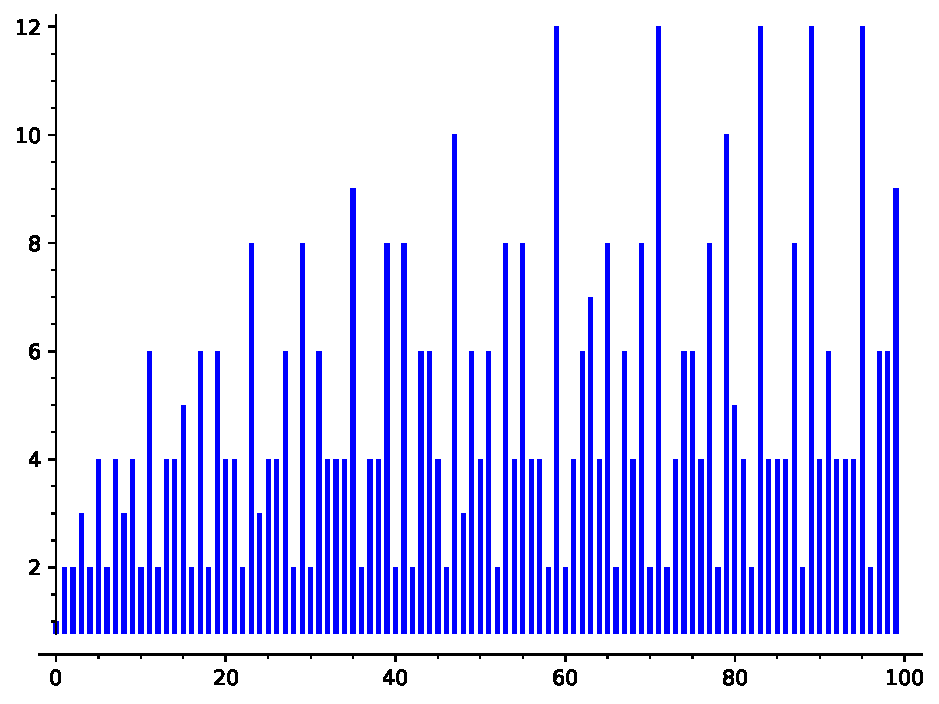
\includegraphics[width=10cm]{Pics/t_plot.pdf}
	\end{center} 
\end{bem}

\begin{defn}
	Sei $\bar{t} : \N \to \R$ die Funktion
	\[
			\bar{t} (n) := \frac{1}{n} \sum_{j=1}^n t(j).
	\]
\end{defn} 

\begin{bem}
	Das Verhalten von $\bar{t}$ erschient viel regelmäßiger zu sein. 
	\begin{center}
	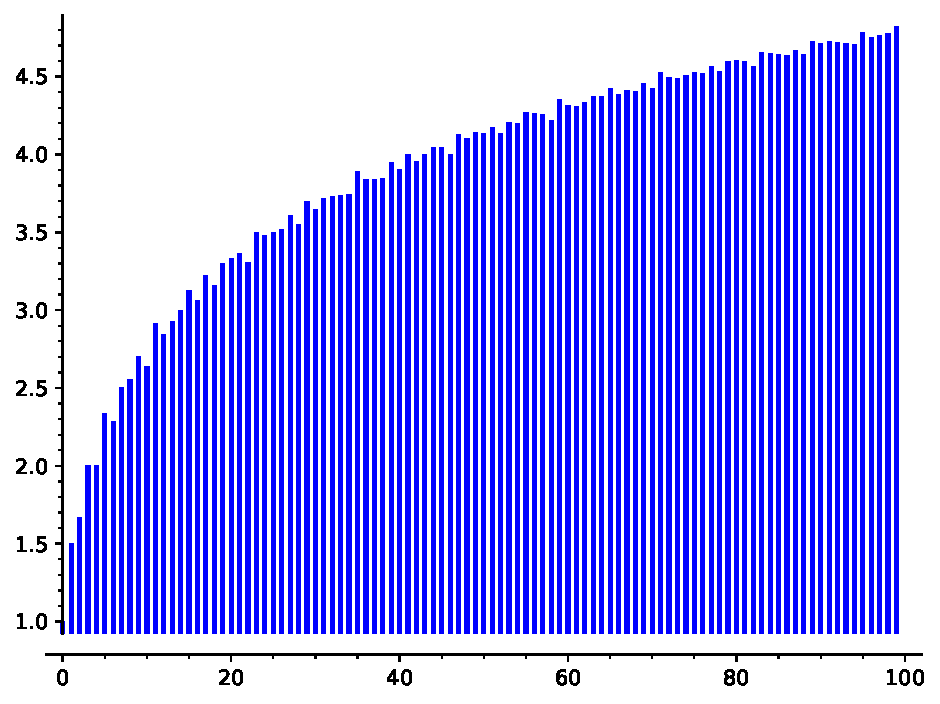
\includegraphics[width=10cm]{Pics/t_bar_plot.pdf}
\end{center} 
\end{bem} 

\begin{defn}
	Für $n \in \N$ nennt man $H_n := \sum_{i=1}^n \frac{1}{i}$ die $n$-te \textbf{harmonische Zahl}. 
\end{defn} 

\begin{thm}
	Es gilt
	\[
		 H_n - 1 \le \bar{t}(n) \le H_n 
	\]
	für alle $n \in \N$. 
\end{thm} 
\begin{proof}
	Man hat 
	\begin{align*} 
		\bar{t} (n) & = \frac{1}{n} \sum_{k=1}^n t(k) 
		\\ & = \frac{1}{n} \sum_{k=1}^n | \setcond{i \in \N}{i \ \text{teilt} \ k}. 
		\\ & = \frac{1}{n} | \setcond{(i,k)}{i,k \in \{1,\ldots,n\}, i \ \text{teilt}  \ k}. 
		\\ & = \frac{1}{n} \sum_{i=1}^n \floor{ \frac{n}{i}}. 
	\end{align*}  
	Aus 
	\[
			\bar{t} (n) = \frac{1}{n} \sum_{i=1}^n \floor{ \frac{n}{i}}
	\]
	ergibt sich einerseits wegen $\floor{ \frac{n}{i}} \le \frac{n}{i}$ die Ungleichung 
	\[
			\bar{t}(n) \le H_n
	\]
	und andererseits wegen $\floor{ \frac{n}{i} } \ge \frac{n}{i} - 1$ die Ungleichung 
	\[
			\bar{t}(n) \ge H_n -1. 
	\]
\end{proof} 

\begin{bem}
	Mit Hilfe der Analysis (IT-3) kann gezeigt werden, dass $H_n= \Theta(\ln n)$ gilt. Also ist 
	\[
		\bar{t}(n) = \Theta(\ln n). 
	\]
\end{bem} 

\begin{bem}
	Der vorige Beweis basiert auf der Präsentation in \cite[Kap.~25, Abs.~4]{AZ02}. 
\end{bem} 

\section{Schubfachprinzip} 

\subsection{Das Prinzip} 

\begin{bem}
	Das Schubfachprinzip ist ein nützliches Mittel, kombinatorische und diskrete  Existenzaussagen zu verifizieren. 
\end{bem} 

\begin{defn}
	Aufrunden und Abrunden sind Abbildungen $\R \to \Z$, die folgendermaßen definieren werden: 
	\begin{align*}
			\ceiling{x} & := \min \setcond{k \in \Z}{x \le k}
			\\ \floor{x} & := \max \setcond{k \in \Z}{x \ge k}. 
	\end{align*} 
\end{defn} 


\begin{prop}[Schubfachprinzip: starke Form] \label{prop:schubfach:stark}
	Seien $X, Y$ nichtleere endliche Mengen. Dann gibt es für jede Abbildung $f: X \to Y$ ein $y \in Y$ mit 
	\[
		|f^{-1} (\{y\})|  \ge  \ceiling{\frac{|X|}{|Y|}} 
	\]
\end{prop} 
\begin{proof} $X$ ist disjunkte Vereinigung der Mengen 
	\[
			X = \bigcup_{y \in Y} f^{-1}(\{y\}) 
	\]
	Somit ist 
	\[
		|X| = \sum_{y \in Y} | f^{-1}(\{y\}) | 
	\]
	Es folgt: 
	\[
		|X| \le |Y| \max_{y \in Y} |f^{-1}(\{y\}) |. 
	\]
	Das bedeutet, dass für das $y \in Y$ mit der maximalen Kardinalität $|f^{-1}(\{y\}) |$, die Ungleichung 
	\[
			|f^{-1}(\{y\})| \ge \frac{|X|}{|Y|}
	\]
	erfüllt ist. Da die Kardinalität auf der linken Seite eine ganze Zahl ist, kann die Ungleichung durch das Aufrunden des Quotienten auf der rechten Seite verstärkt werden: 
	\[
			|f^{-1}(\{y\})| \ge \ceiling{\frac{|X|}{|Y|}}.
	\]
\end{proof} 


\begin{bsp}
	In einem Haus mit $10$ Wohungen und insgesamt $21$ Bewohner:innen, wohnt in einer Wohnung mindestens $3$ Bewohner:innen. 
\end{bsp} 

\begin{kor}[Schubfachprinzip: schwache Form] 
	Seien $X, Y$ endliche Mengen mit $|X| > |Y| >0$. Dann gibt es für jede Abbildung $f : X \to Y$ verschiedene $x',x''\in X$ mit $f(x')=f(x'')$. 
\end{kor} 
\begin{proof}
	Die Behauptung folgt durch eine direkte Anwendung von Proposition~\ref{prop:schubfach:stark}.
\end{proof} 

\subsection{Einfache Beispiele} 

\begin{aufg}
	Zeigen Sie, dass jede Färbung der Seitenflächen eines (dreidimensionalen) Würfels mit zwei Farben ein Paar von Seitenflächen besitzt	die benachbart sind ($=$ eine gemeinsame Kante haben) und die gleiche Farbe haben. 
\end{aufg}

\begin{aufg}
	Zeigen Sie, dass jede Färbung der Seitenflächen eines (dreidimensionalen) Würfels mit zwei Farben vier Seitenflächen $A,B,C,D$ besitzt, bei denen $A$ und $B$ sowie $C$ und $D$ gleich gefärbt wurden. 
\end{aufg} 

\begin{aufg}
	$30$ Schüler:innen, darunter auch Fritzchen, haben eine Klassenarbeit geschrieben. In der Klassenarbeit hat Fritzchen $13$ Fehler gemacht, und alle anderen Schülerinnen weniger. Zeigen Sie, dass drei der Schüler:innen die gleiche Anzahl der Fehler gemacht haben. 
\end{aufg}  

\begin{aufg}
	Zeigen Sie, dass in einem Fußballturnier mit $n \in \N$ Mannschaften ($n \ge 2$) in jedem Zeitpunkt man zwei Mannschaften findet, die zu diesem Zeitpunkt die gleiche Anzahl der Spiele gespielt haben. 
\end{aufg} 

\subsection{Der Satz von Erd\H{os}-Szekeres}


\begin{thm}[Erd\H{os}-Szekeres] 
	Seien $m, n \in \N$, sei $k=mn+1$ und sei $a_1,\ldots,a_k$ Folge paarweise verschiedener reeller Zahlen. Dann besitzt die Folge eine ansteigende Teilfolge 
	\[
			a_{i_1}  < a_{i_2} < \cdots < a_{i_{m+1}} \qquad (1 \le i_1 < \cdots < i_{m+1} \le k)
	\]
	der Länge $m+1$ oder eine absteigende Teilfolge 
	\[
		 a_{j_1} > a_{j_2} > \cdots > a_{j_{n+1}} \qquad (1 \le j_1 < \cdots < j_{n+1} \le k)
	\]
	der  Länge $n+1$. 
\end{thm} 
\begin{proof}
	Sei $t_i$ die Länge der längesten ansteigenden Teilfolge, die mit $a_i$ anfängt. Gilt für ein $a_i$ die Ungleichung $t_i \ge m+1$, so besitzt unsere Folge eine ansteigende Teilfolge der Länge $m$. Wir nehmen also an, dass $t_i \le m$ für alle $i=1,\ldots, k$ gilt. Das ergibt dann die Abbildung $a_i \mapsto t_i$, welche die $k$-elementige Menge $\{a_1,\ldots,a_k\}$ auf die Menge $\{1,\ldots,m\}$  Wegen $k=mn+1$ hat man ein einen Wert $s \in \{1,\ldots,m\}$, so dass $f(a_i) = s$ für $n+1$ Zahlen $a_i$ gilt. Seien $a_{j_1}, \cdots ,  a_{j_{n+1}}$ diese $n+1$ Zahlen mit $1 \le j_1 < \cdots < j_{n+1} \le k$. Wir vergleichen nun $a_{j_t}$ und $a_{j_{t+1}}$. Wäre $a_{j_t} < a_{j_{t+1}}$, so hätten wir eine ansteigende Folge der Länge $s+1$ die mit $a_{j_t}$ beginnt, was der Wahl von $a_{j_t}$ widerspricht. Also hat man $a_{j_t} > a_{j_{t+1}}$. Wir erhalten 
	\[
		a_{j_1} > \cdots > a_{j_{n+1}}.
	\]
	Das ist eine absteigende Teilfolge der Länge $n+1$. 
\end{proof} 

\begin{bem}
	``Complete disorder is impossible'' (Theodore S. Motzkin). 
\end{bem} 

\begin{bem}
	Der vorige Beweis basiert auf der Präsentation in \cite{AZ02}. 
\end{bem} 

%\subsection{Untere Scrhanken an Ramsey-Zahlen} 

%\begin{defn}
%	Für eine Menge $V$ heißt ein Paar $G=(V,E)$ mit $E \subseteq \binom{V}{2}$ ein (ungerichteter) Graph mit Knotenmenge $V$ und der Kantenmenge $E$. 
%\end{defn} 

%\begin{defn}
%		Ist $E= \binom{V}{2}$, so nennt man den Graphen $G$ vollständig. Einen vollständigen Graphen auf $n \in \N$ knoten bezeichnet man oft als $K_n$. 
%\end{defn} 

%\begin{defn} 
%		Gelten für Graphen $G_1 = (V_1,E_2)$ und $G_2= (V_2,E_2)$ die Inklusionen $V_1 \subseteq V_2$ und $E_1 \subseteq E_2$, so heißt $G_1$ Teilgraph von $G_2$. 
%\end{defn} 

%\begin{defn} 
%		Eine Abbildung $c : E \to \{1,\ldots,t\}$ mit $t \in \N$ nennt man Färbung der Kanten von $G=(V,E)$ mit $t$ Farben. Gilt für einen Teilgraphen $G'= (V',E')$ von $G$, dass alle Kanten von $G'$ die gleiche Farben bzgl. $c$ haben, so nennt man den Teilgraphen $G'$ monochromatisch. 
%\end{defn} 

%\begin{defn} 
%	Die Ramsey Zahl $R(t,t)$ ist die kleinste Zahl $n \in \N$ derart, dass jede Färbung von $K_n$ mit zwei Farben eine monochromatische Kopie von $K_t$ besitzt. 
%\end{defn} 

%\begin{bem}
%	A priori ist nicht klar, ob ein solches $n \in \N$ überhaupt existiert, aber das wurde gezeigt (vgl. Ramsey-Theorem unten). 
%\end{bem} 

%\begin{bsp}
%	$R(3,3) = 6$. 
%\end{bsp} 

%\begin{thm}[Ramsey-Theorem]
%	Es gilt $R(t,t) < 4^{t-1}$ für alle $t \in \N$. 
%\end{thm} 

%\begin{bem}
%	``Complete disorder is impossible'' (Theodore S. Motzkin). 
%\end{bem} 


%\begin{thm}
%	Es gilt $R(t,t) > \floor{2^{t/2}}$ für alle $t \in \N$. 
%\end{thm} 
%\begin{proof} IM AUFBAU 
%\end{proof} 

%\section{Weitere Themen}

%Partitionen in\cite[Abschnitt~1.4]{Tit19} und Verteilungen in  \cite[Abschnitt~1.5]{Tit19}. 


